\documentclass[english,11pt]{beamer}

\DeclareMathOperator{\Cov}{Cov}
\DeclareMathOperator{\Var}{Var}
\DeclareMathOperator{\E}{\mathbb{E}}
\DeclareMathOperator{\Proba}{\mathbb{P}}

\newcommand{\Covb}[2]{\ensuremath{\Cov\!\left[#1,#2\right]}}
\newcommand{\Eb}[1]{\ensuremath{\E\!\left[#1\right]}}
\newcommand{\Pb}[1]{\ensuremath{\Proba\!\left[#1\right]}}
\newcommand{\Varb}[1]{\ensuremath{\Var\!\left[#1\right]}}

% norm
\newcommand{\norm}[1]{\| #1 \|}

\newcommand{\indep}{\rotatebox[origin=c]{90}{$\models$}}





\usepackage{mathptmx,amsmath,amssymb,graphicx,bibentry,bbm,babel,ragged2e}

\makeatletter

\newcommand{\noun}[1]{\textsc{#1}}
\newcommand{\jitem}[1]{\item \begin{justify} #1 \end{justify} \vfill{}}
\newcommand{\sframe}[2]{\frame{\frametitle{#1} #2}}

\newenvironment{centercolumns}{\begin{columns}[c]}{\end{columns}}
%\newenvironment{jitem}{\begin{justify}\begin{itemize}}{\end{itemize}\end{justify}}

\usetheme{Warsaw}
\setbeamertemplate{footline}[text line]{}
\setbeamercolor{structure}{fg=purple!50!blue, bg=purple!50!blue}

\setbeamersize{text margin left=15pt,text margin right=15pt}

\setbeamercovered{transparent}


\@ifundefined{showcaptionsetup}{}{%
 \PassOptionsToPackage{caption=false}{subfig}}
\usepackage{subfig}

\usepackage[utf8]{inputenc}
\usepackage[T1]{fontenc}



\makeatother

\begin{document}


\title{Structural Segregation: Assessing the impact of South African Apartheid on Underlying Dynamics of Interactions between Networks and Territories}

\author{J.~Raimbault$^{1,2,\ast}$ and \noun{S.~Baffi}$^{1}$\\
$^{\ast}$\texttt{juste.raimbault@polytechnique.edu}
}


\institute{$^{1}$UMR CNRS 8504 G{\'e}ographie-cit{\'e}s\\
$^{2}$UMR-T IFSTTAR 9403 LVMT\\
}


\date{ECTQG 2017 - York\\\smallskip
Session 6B  - Accessibility\\\smallskip
September 10th 2017
}

\frame{\maketitle}





%%%%%%%%%%%%%%%%%%%
%% ABSTRACT
%\textbf{Keywords : }\textit{South Africa ; Network-Territories Interactions ; Railway Network ; Spatio-temporal Causality}


%\paragraph{Networks and Territories}

%Transportation Networks can be leveraged as a powerful socio-economic control tool, with even more significant outcomes when it percolates to their interaction with territories. The case of South Africa is an accurate illustration, as \cite{baffi:tel-01389347} shows that during apartheid railway network planning was used as a racial segregation tool by shaping strongly constrained mobility and accessibility patterns. We propose to investigate the potential \emph{structural} properties of this historical process, by focusing on dynamical patterns of interactions between the railway network and city growth. More precisely, we try to establish if the segregative planning policies did actually modify the trajectory of the coupled system, what would correspond to deeper and wider impacts. 

%\paragraph{Network Measures}

%We use a comprehensive database covering the full South African railway network from 1880 to 2000 with opening and closing dates for each station and link, together with a city database spanning from 1911 to 1991 for which consistent ontologies for urban areas have been ensured. %~(Citation database)\cite{}. %TODO cit. database ?
 %First, a dynamical study of network measures seem to confirm the hypothesis: a trend rupture in closeness centrality (defined for a node as the average travel time to other nodes) at a roughly constant network size evolution, at a date corresponding to the beginning of official segregative policies, suggests that the planning process after this date had in the best case no global effect on network performance, and in the worst case had intended negative effects on accessibility with the aim to physically segregate more.
 

%\paragraph{Causality patterns}

%We then turn to dynamical interactions between the railway network and city growth. For that, we study Granger causalities, in the large sense of correlations between lagged variables, estimated between cities growth rates and accessibility differentials due to network growth. %, for all cities and urban areas having a connection to the network.
% We test both travel-time and population weighted accessibilities, for varying values of distance decay parameter. %Lagged correlations are fitted on varying length time windows, to test for potentially varying stationarity scales.
%  We find that results are significant with travel-time accessibility only, autocorrelation dominating with weighted accessibility. A time-window of 30 years appears to be a good compromise between the number of significant correlations ($p<0.1$ for a Fisher test) and the absolute correlation level across all lags and distance decays, what should correspond roughly to the time-stationarity scale of the system.% We observe furthermore a phase transition when distance decay increases, revealing the shift between the spatial scale of urban areas and the scale of the country, what gives local spatial stationarity scale.
%  We obtain therethrough clear causality patterns, namely an inversion of the Granger causality (lagged correlation up to 0.5 for several values of distance decay), from accessibility causing population growth with a lag of 10-20 years before the apartheid (1948), to the opposite after the apartheid (lag 20 years). We interpret these as \emph{Structural segregation}, i.e. a significant impact of planning policies on dynamics of interactions between networks and territories. Indeed, the first regime corresponds to direct effect of transportation on migrations in a free context in opposition to the second one. Further work should consist in similar study with more precise socio-economic variables, for example quantifying directly segregation patterns.









%%%%%%%%%%%%%%%%%
\section{Introduction}
%%%%%%%%%%%%%%%%%



\sframe{Technical artefacts sublimate human madness}{

\centering

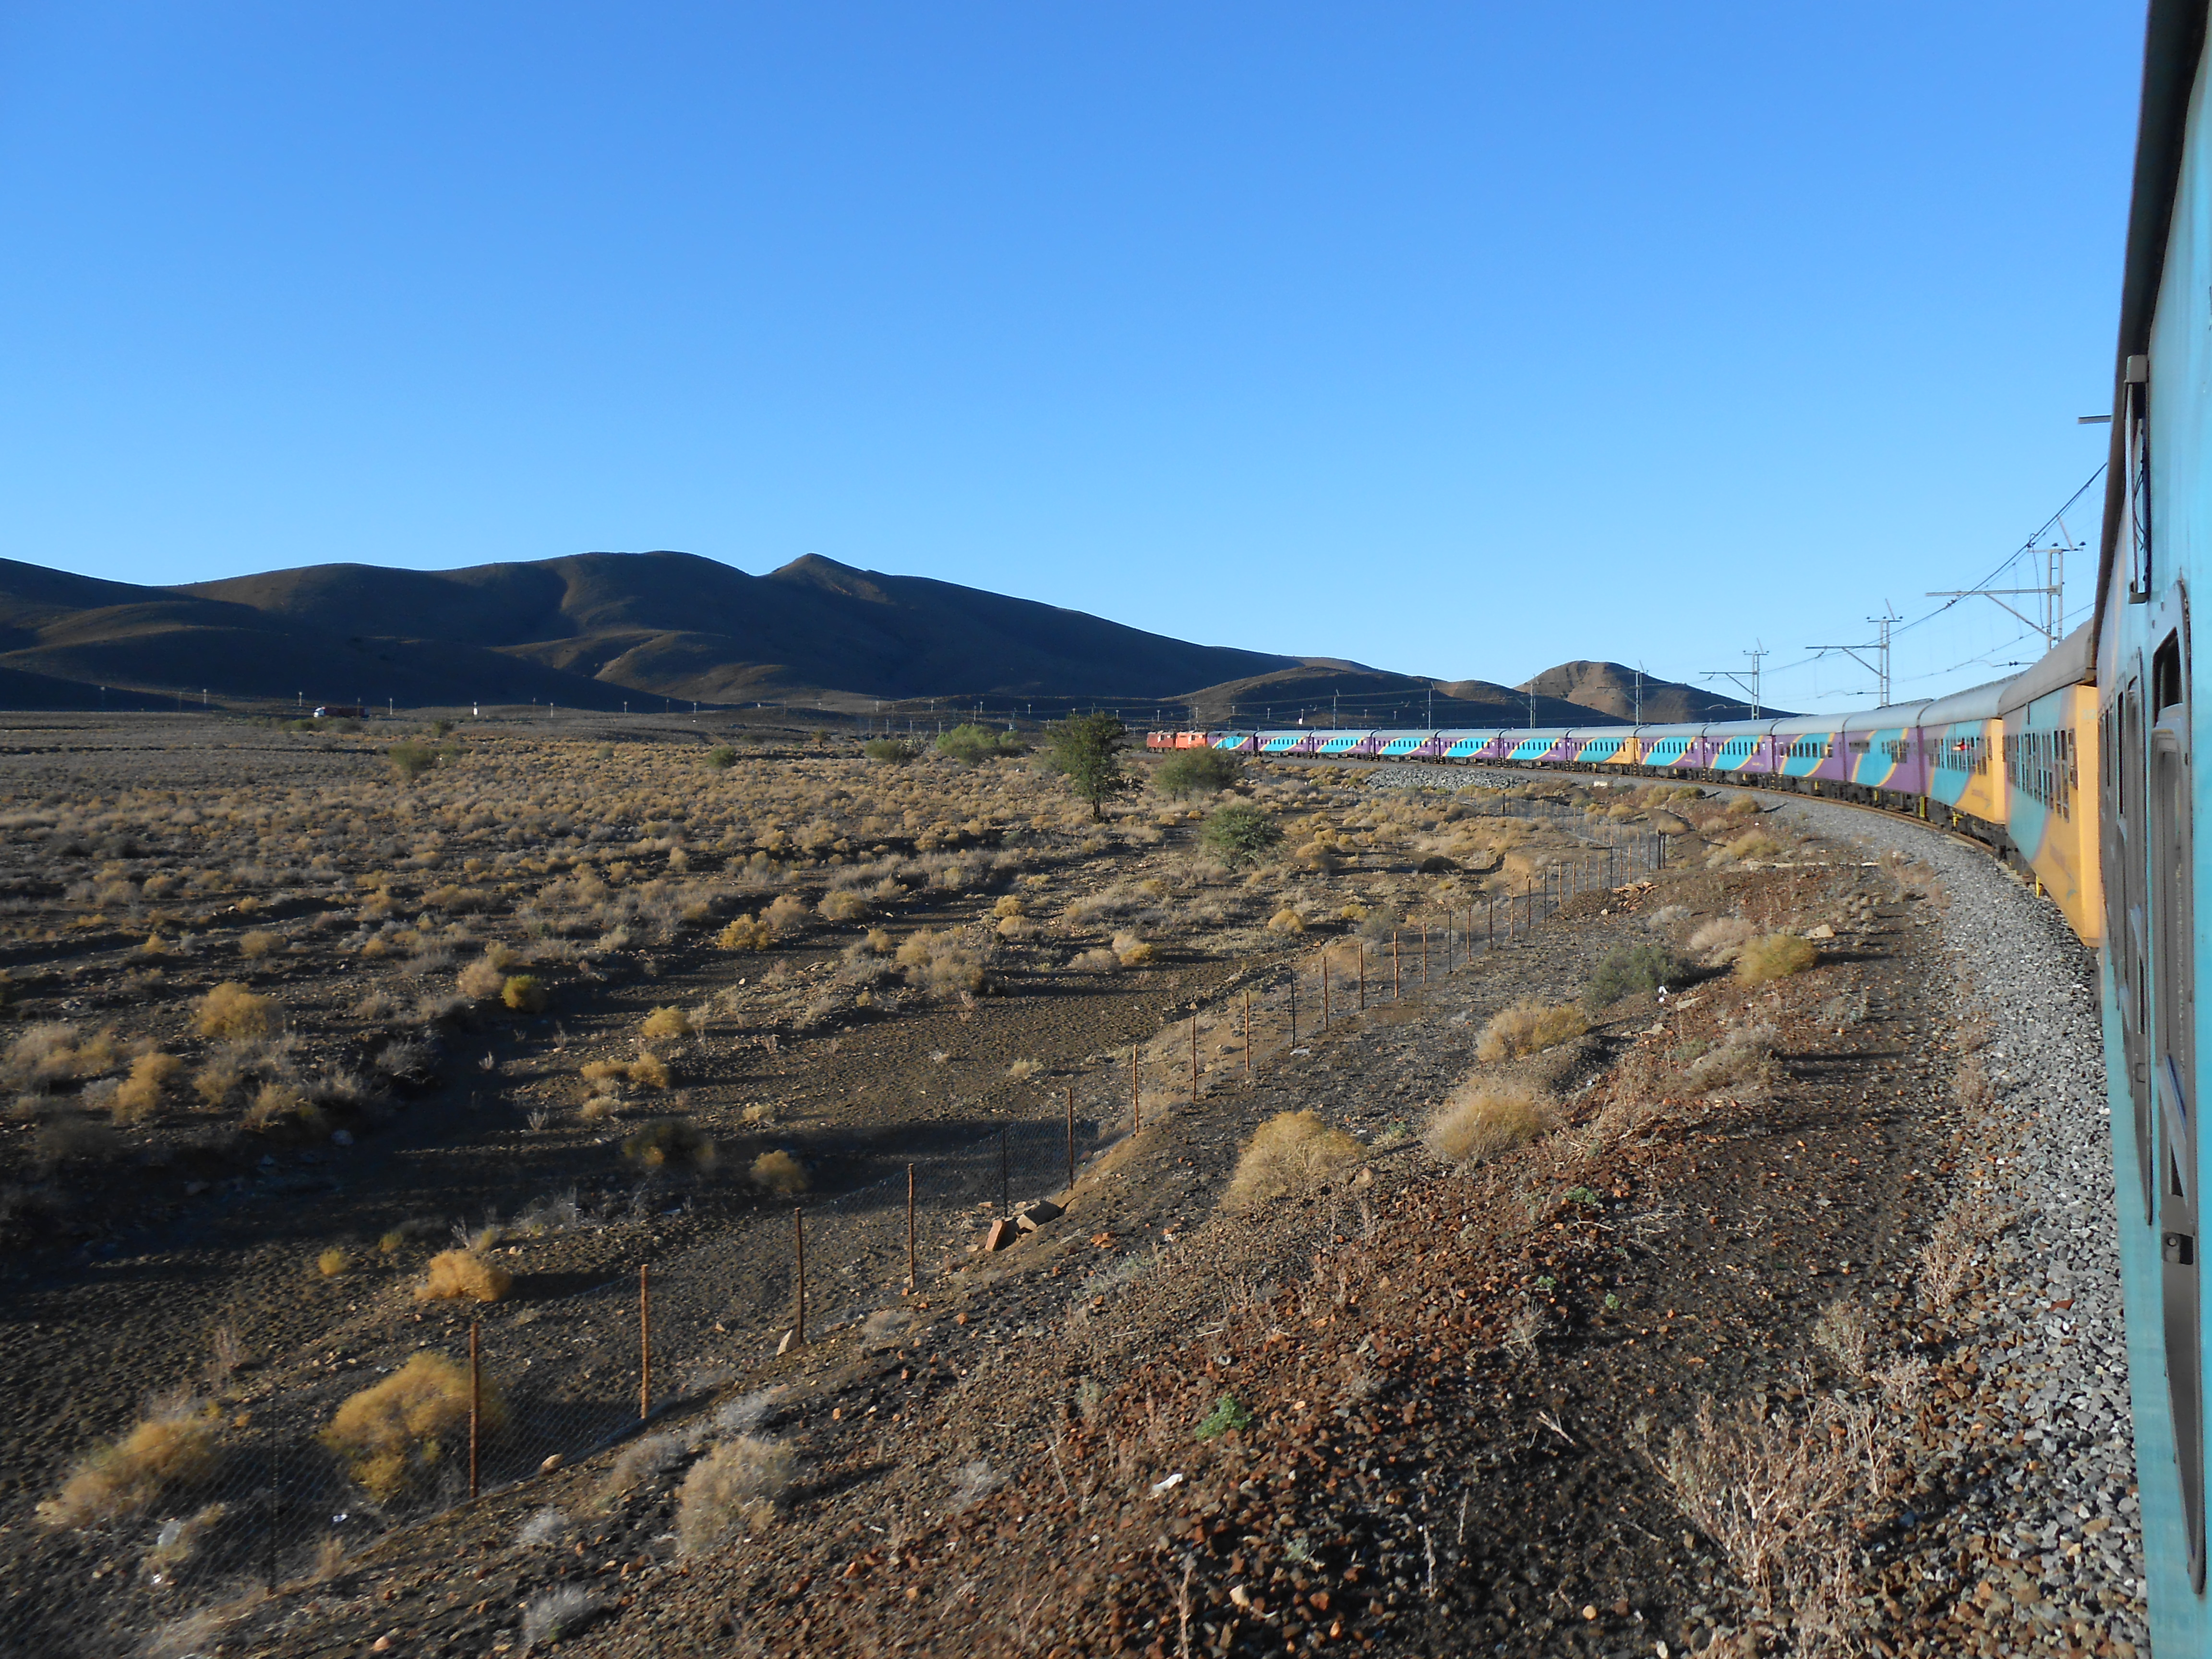
\includegraphics[width=0.4\textwidth]{figures/DSCN0619}\hspace{0.2cm}
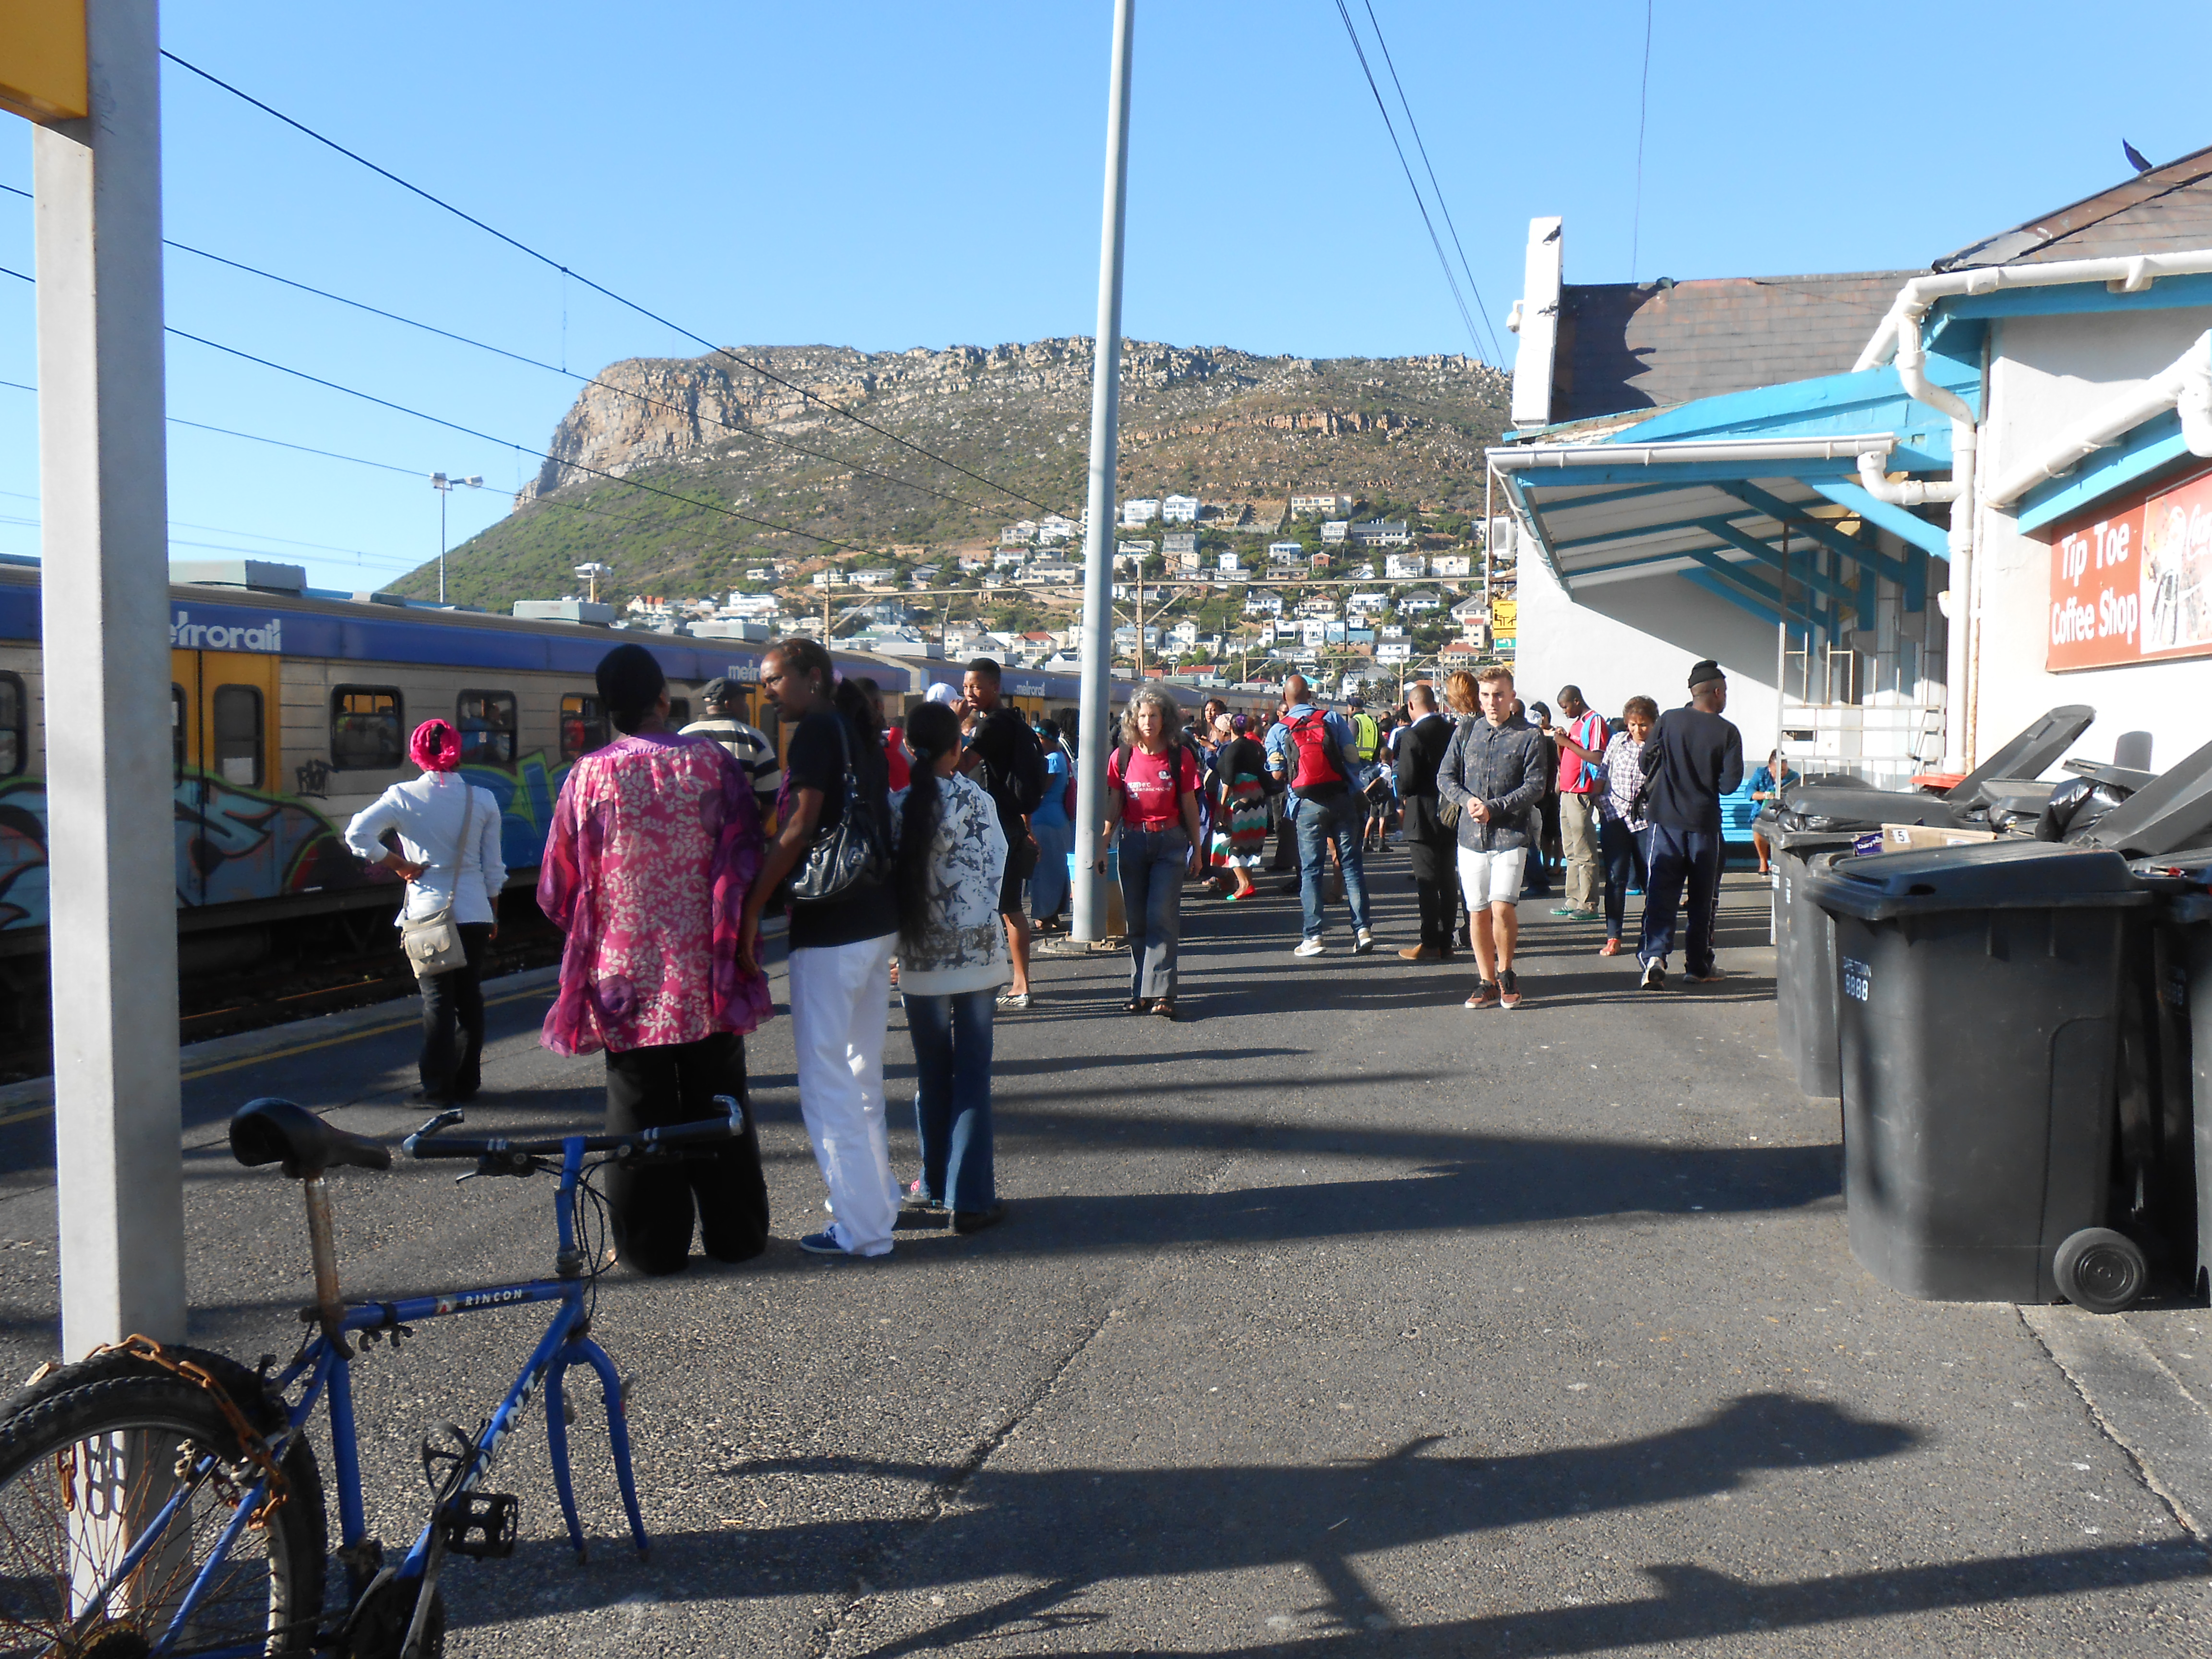
\includegraphics[width=0.4\textwidth]{figures/DSCN1893}\\
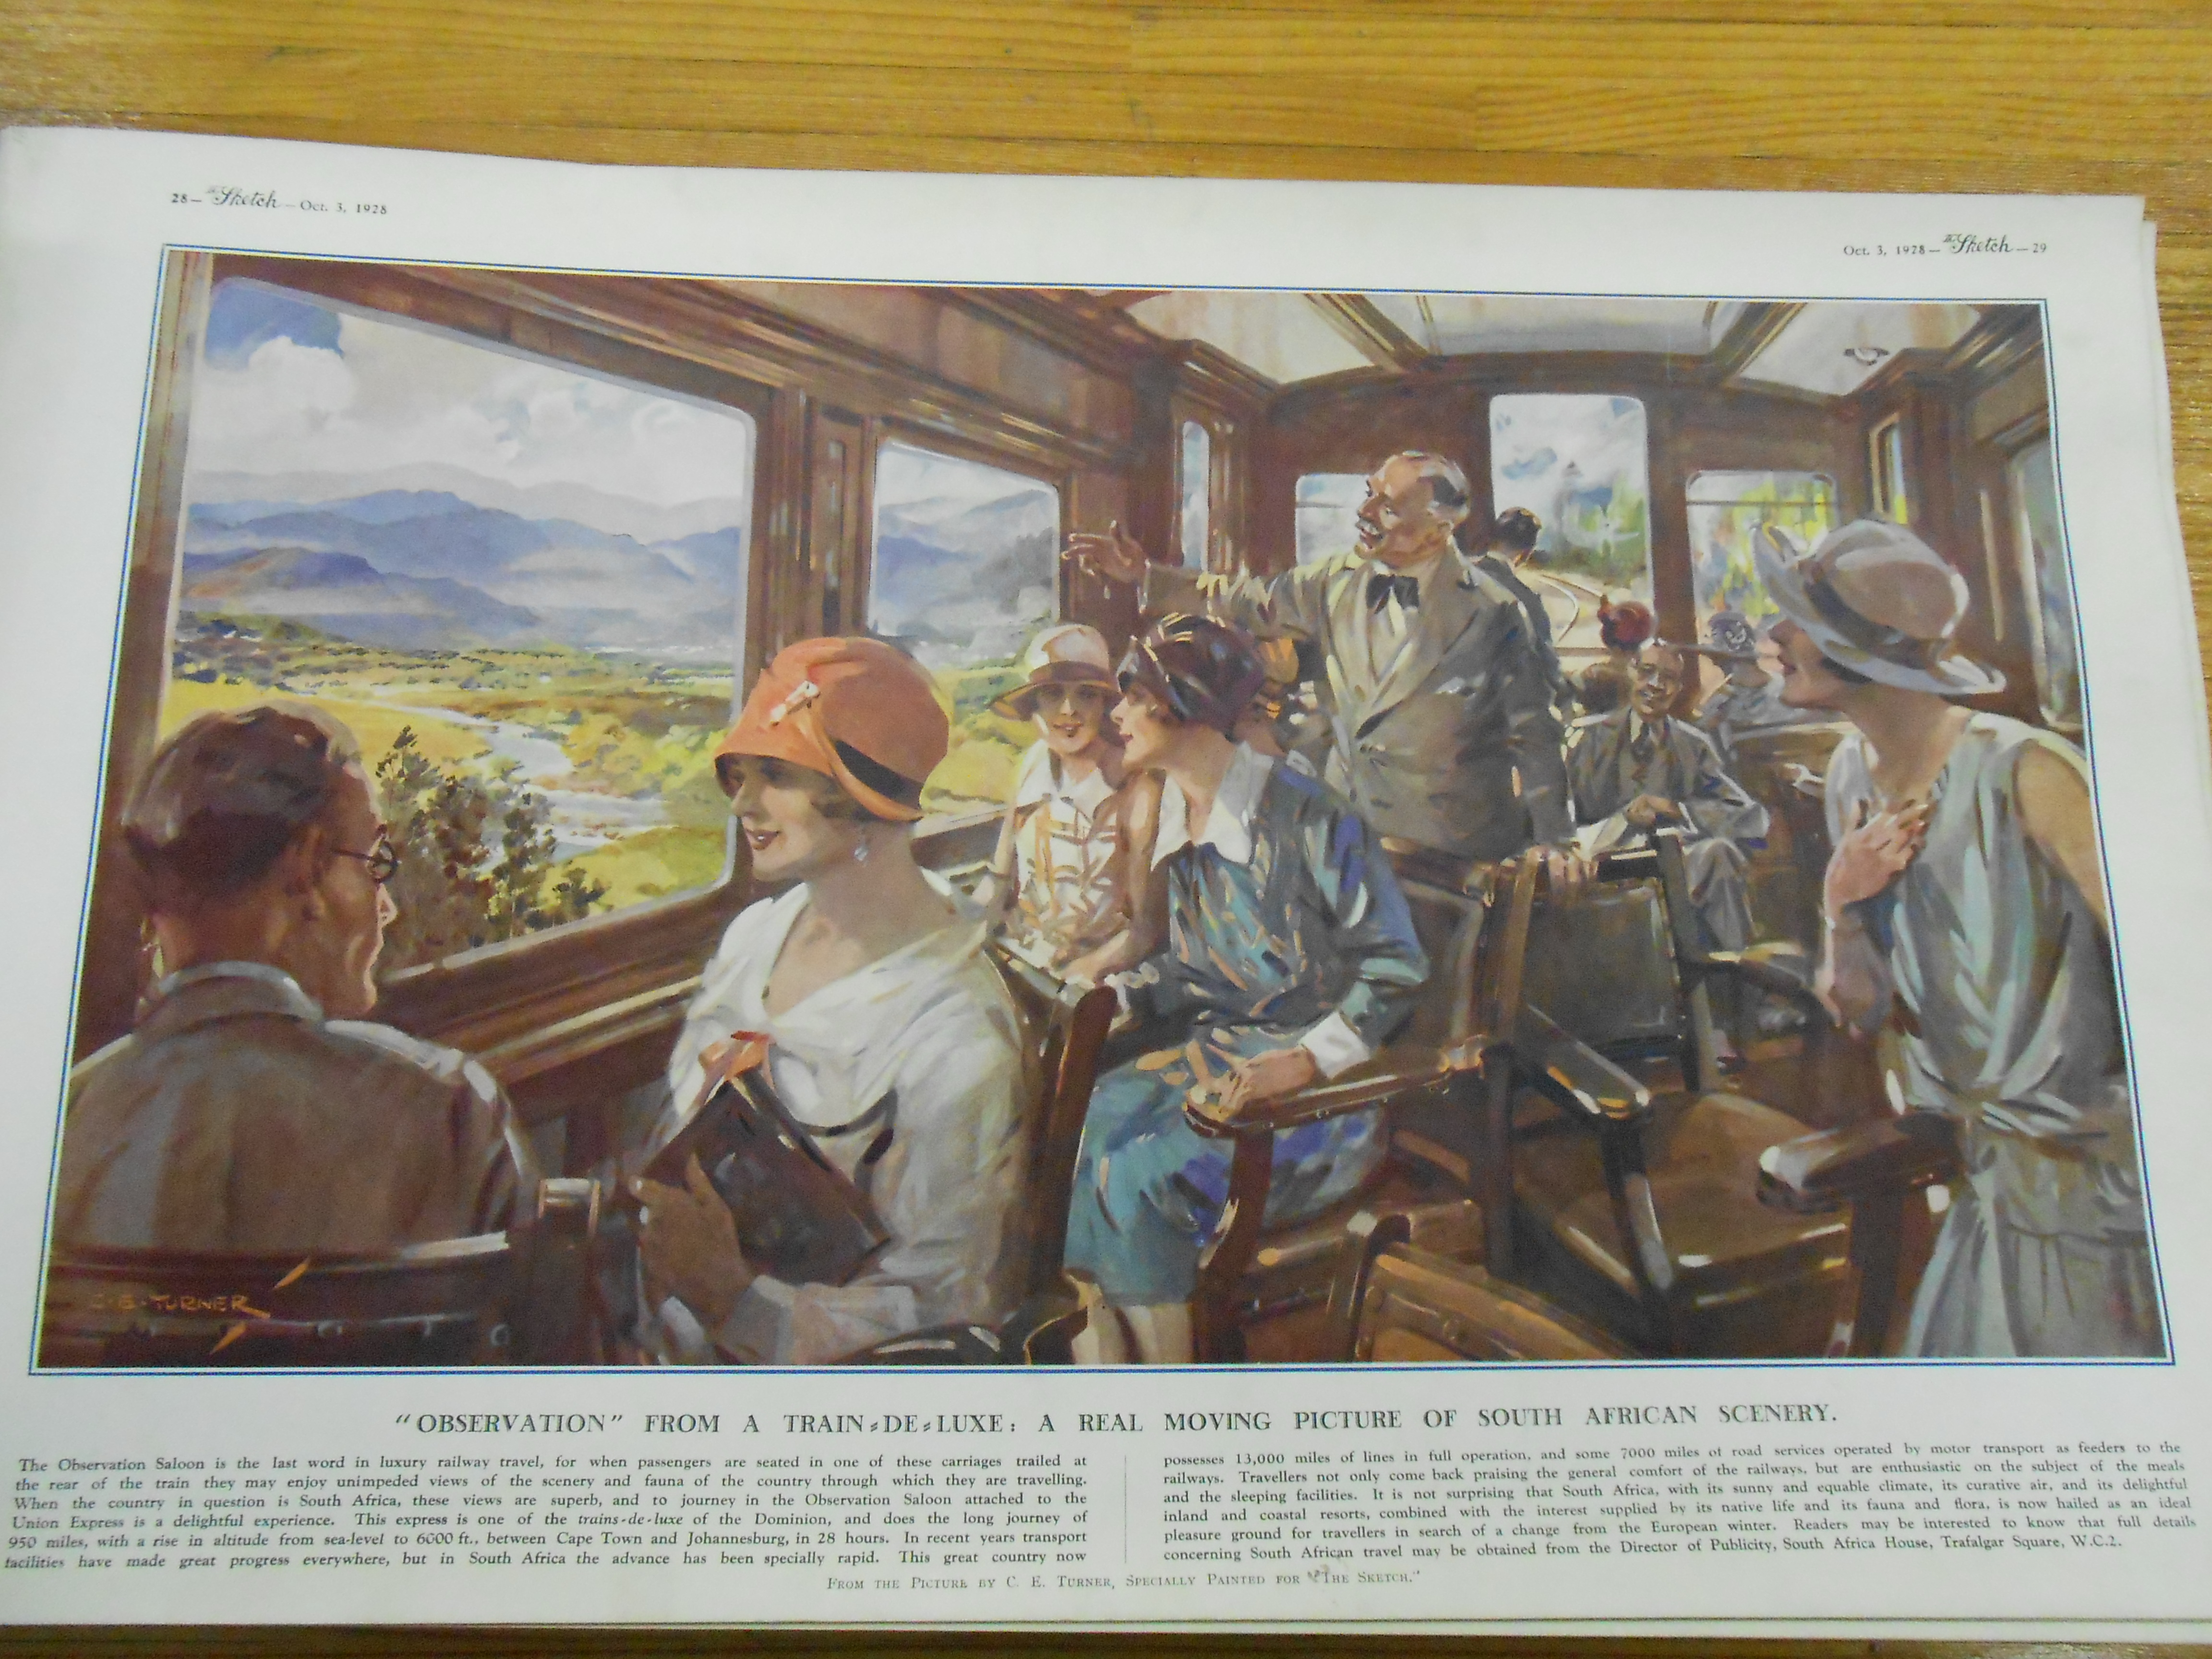
\includegraphics[width=0.4\textwidth]{figures/DSCN0828}\hspace{0.2cm}
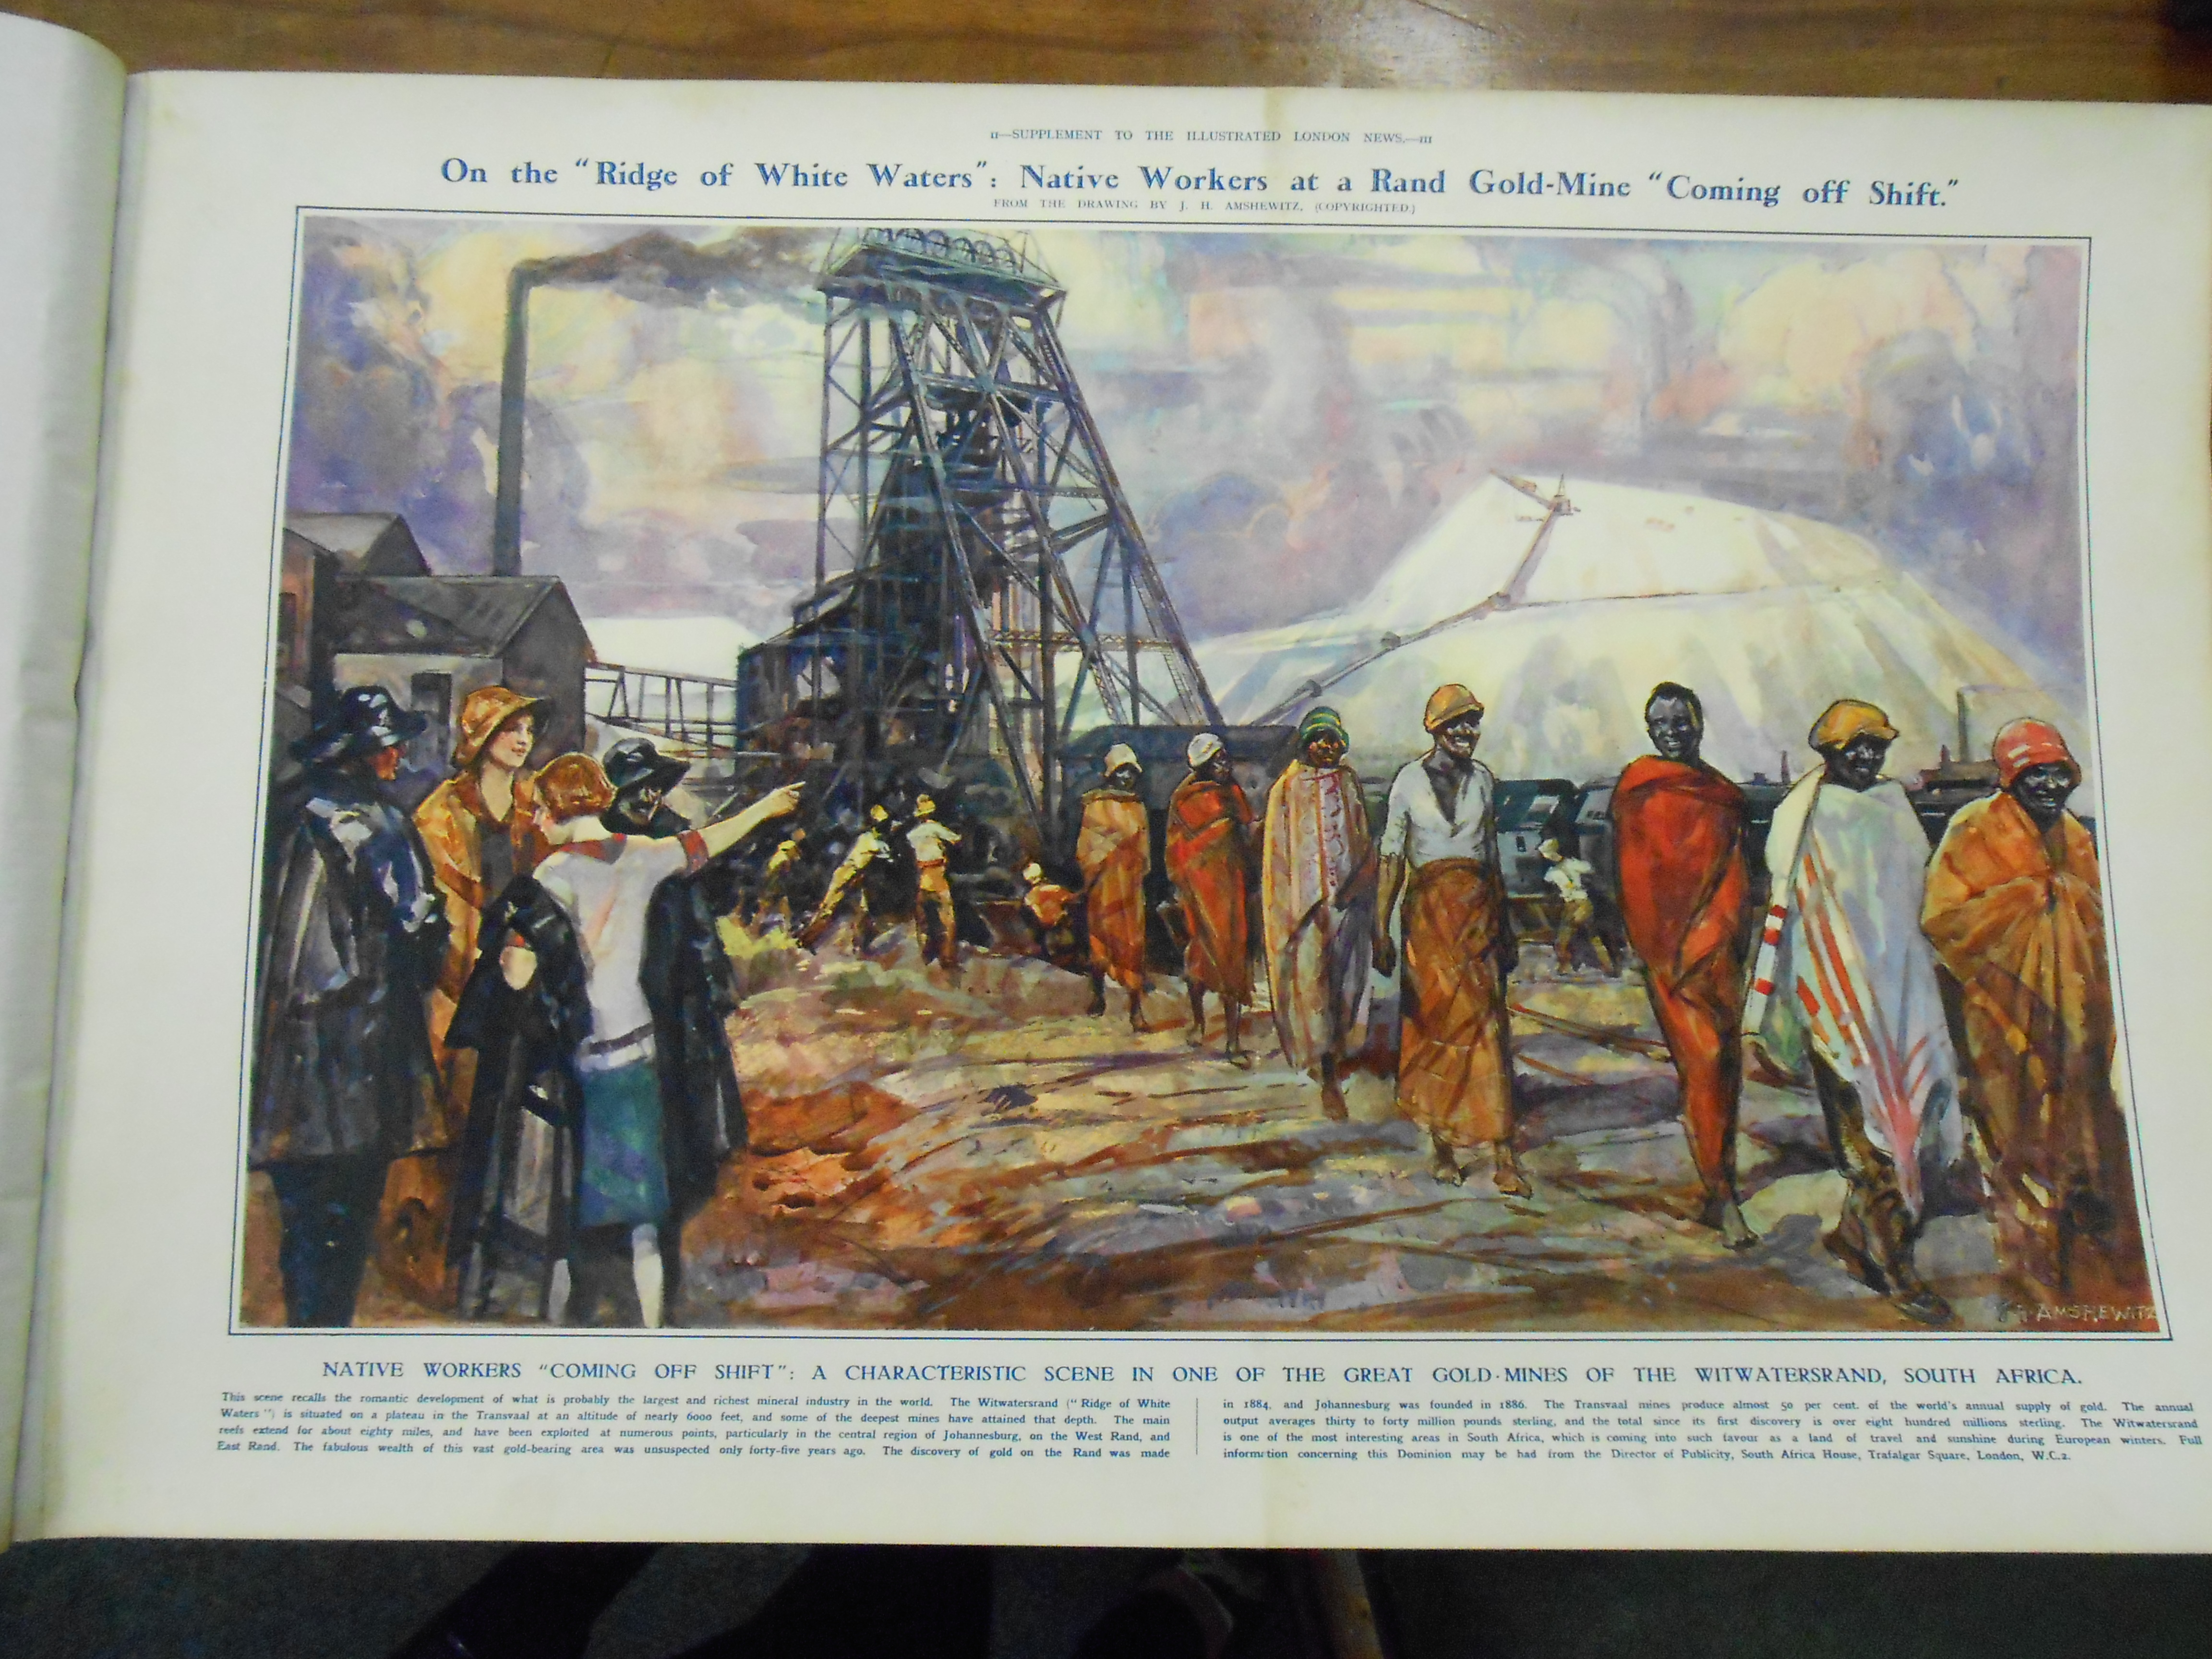
\includegraphics[width=0.4\textwidth]{figures/DSCN0839}


}


\sframe{Context}{

}


\sframe{Interactions between Networks and Territories in South Africa}{

\textit{The de-structuring effects of the segregation laws during apartheid}

\smallskip

\centering

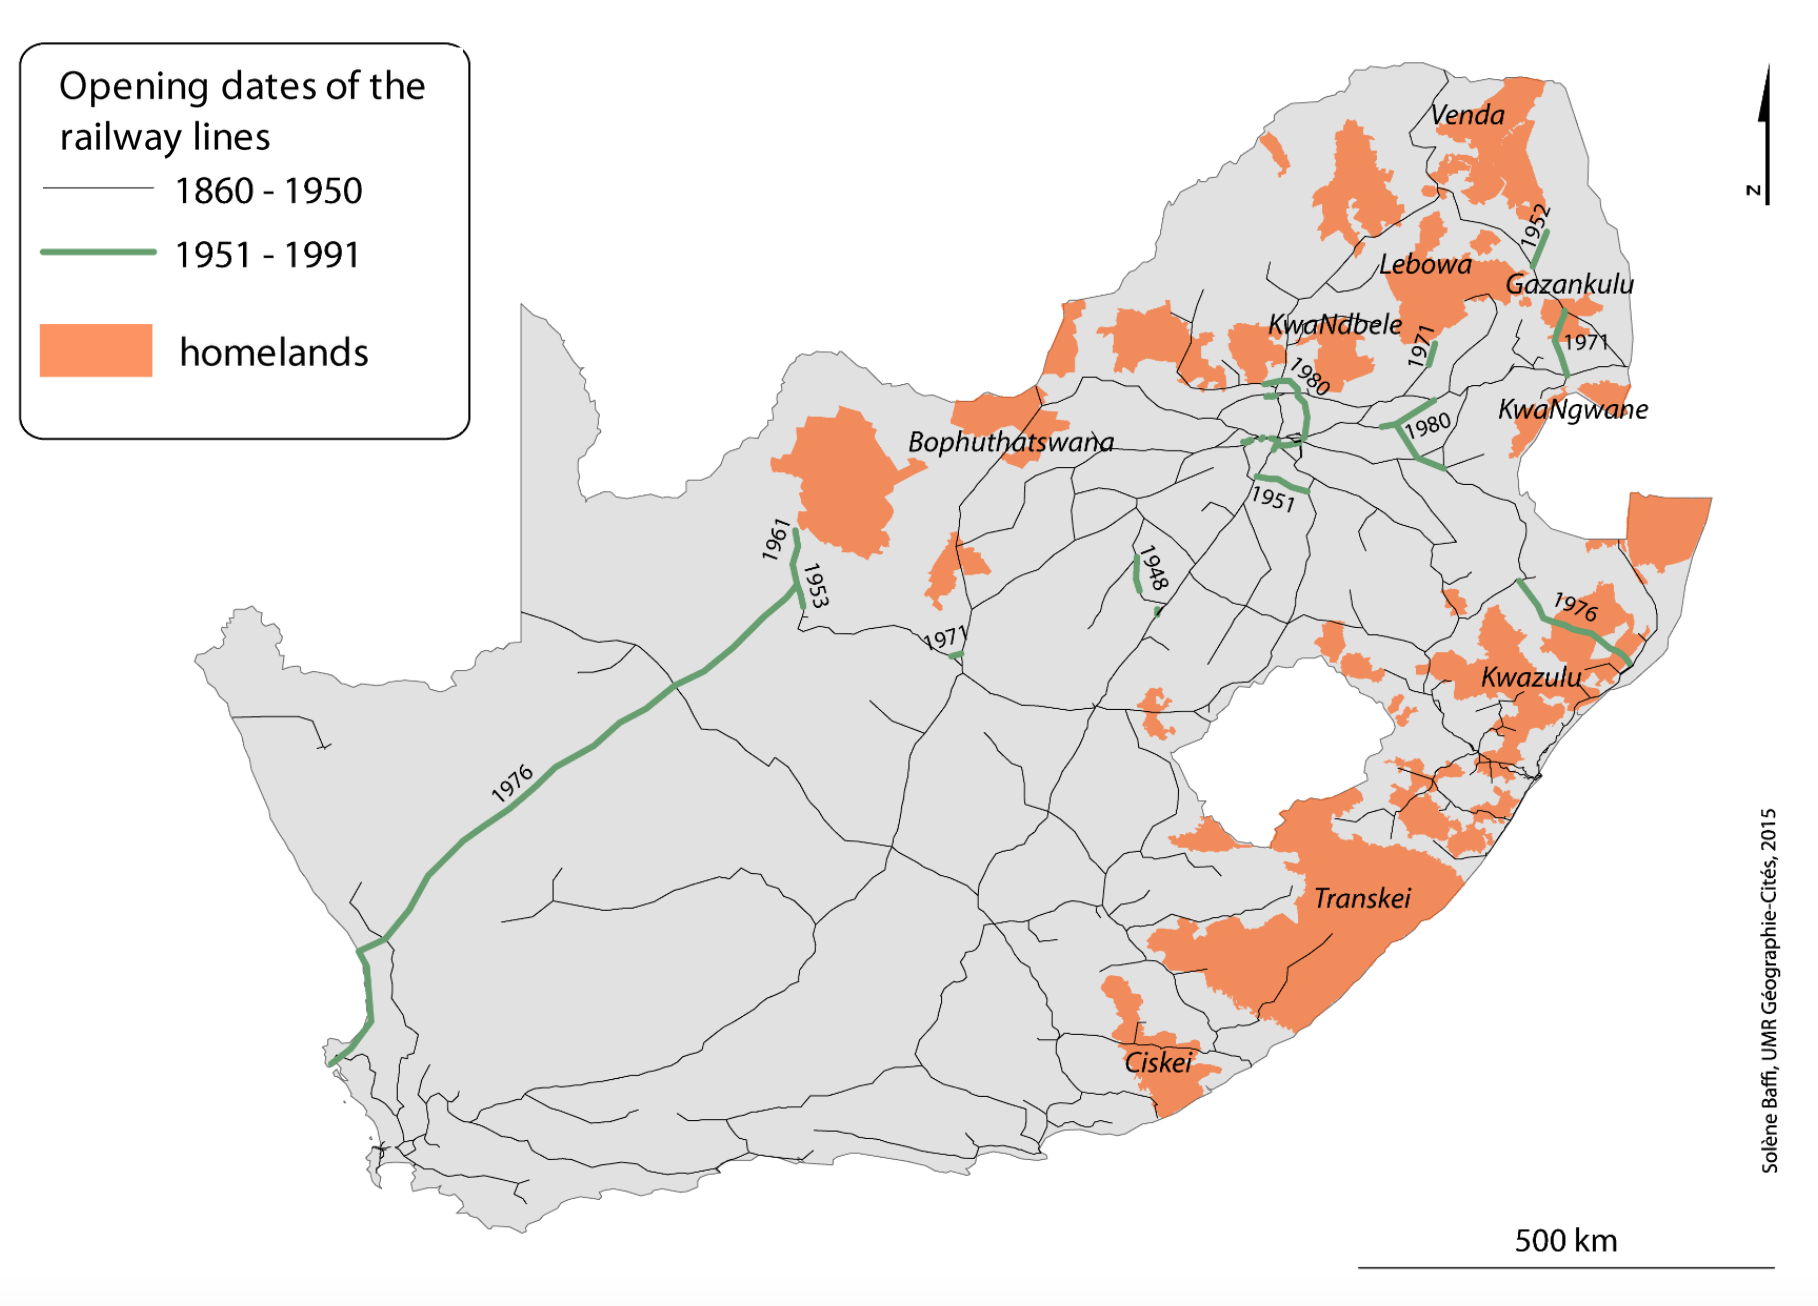
\includegraphics[width=0.8\textwidth]{figures/homelands}

}



%%%%%%%%%%%%%%%%%
\section{Methods and Results}
%%%%%%%%%%%%%%%%%


\sframe{Network Analysis}{

\textit{Connectivity to the railway network : a specific relationship between urban hierarchy and centrality}

\smallskip

\centering

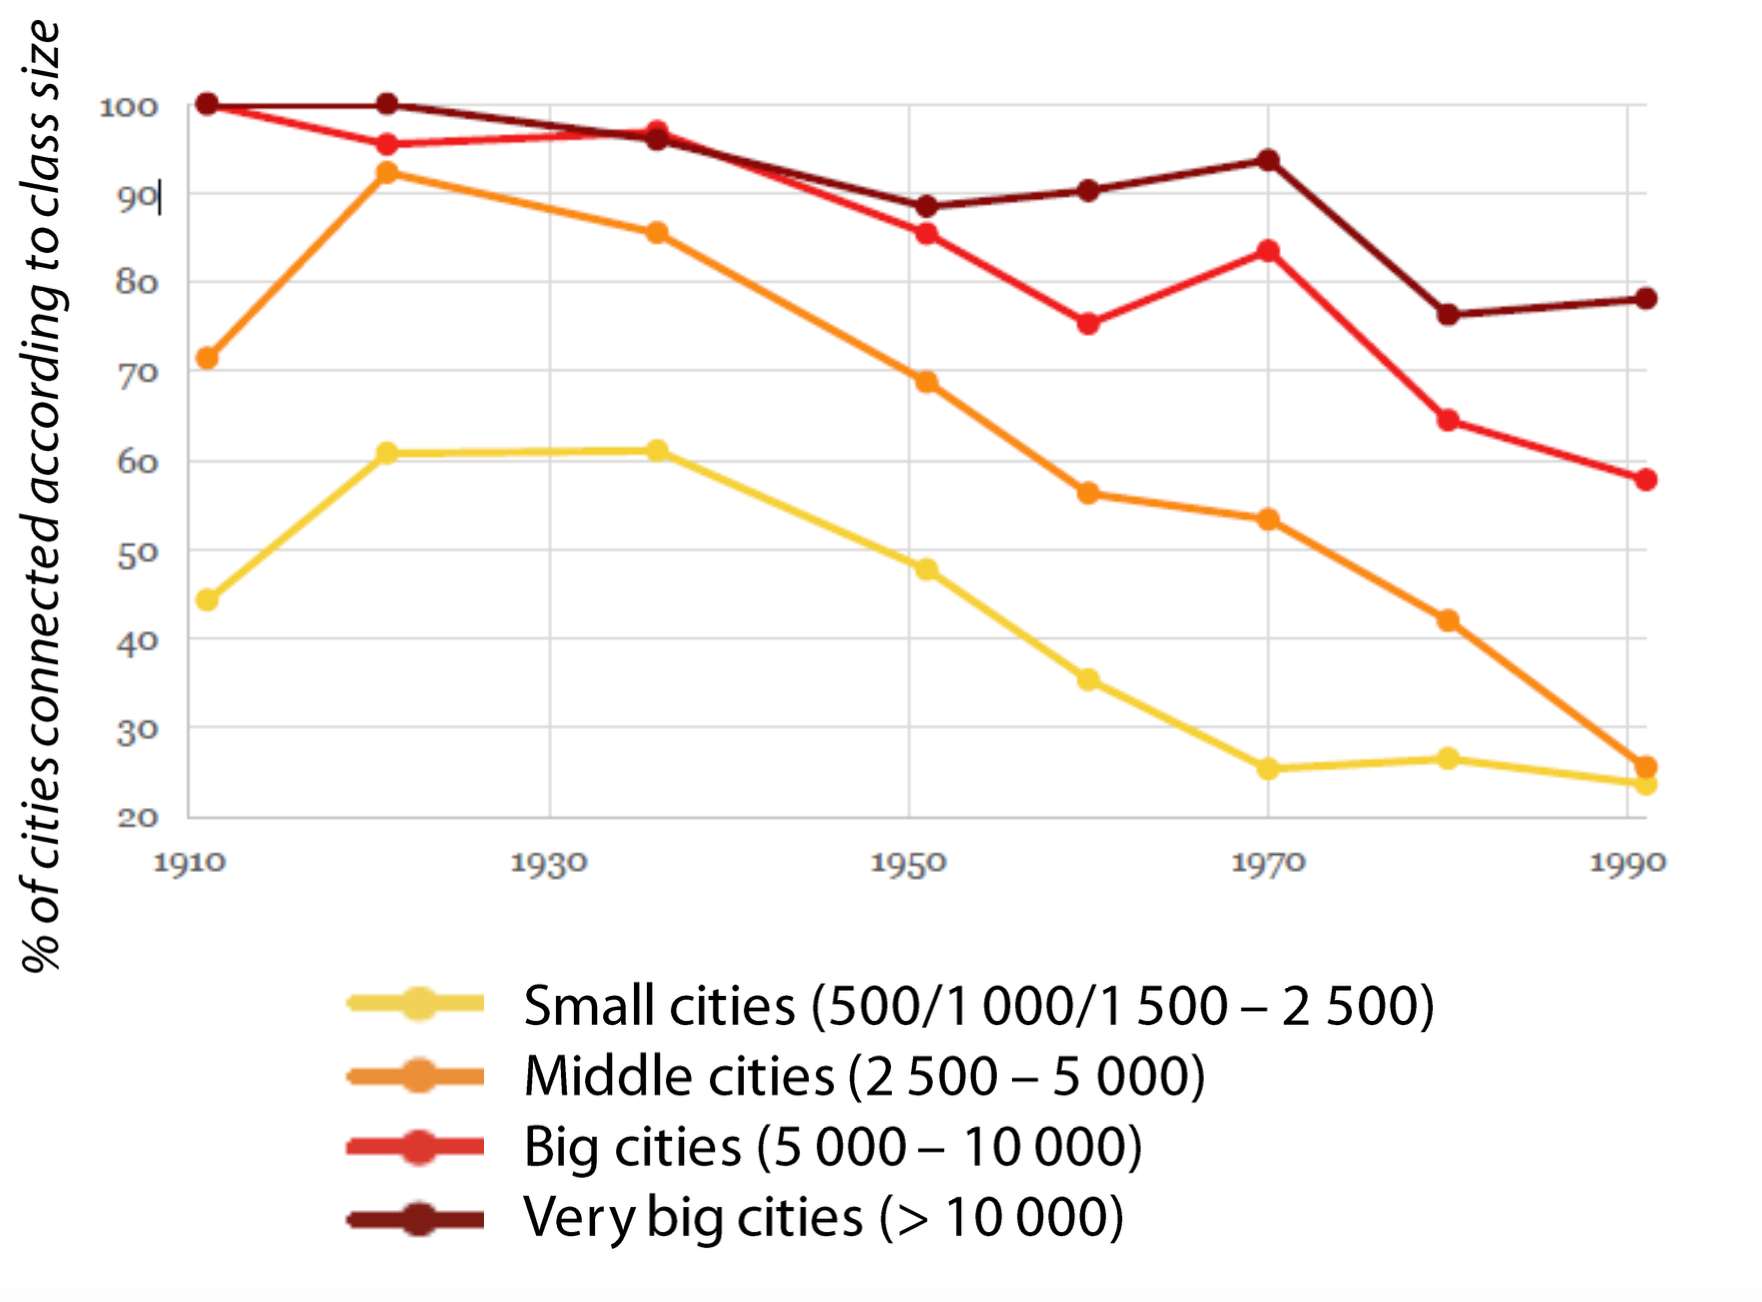
\includegraphics[width=0.8\textwidth]{figures/networkconnection}


}




\sframe{Network Analysis}{

\textit{Evolution of Network measures}

\smallskip

\centering

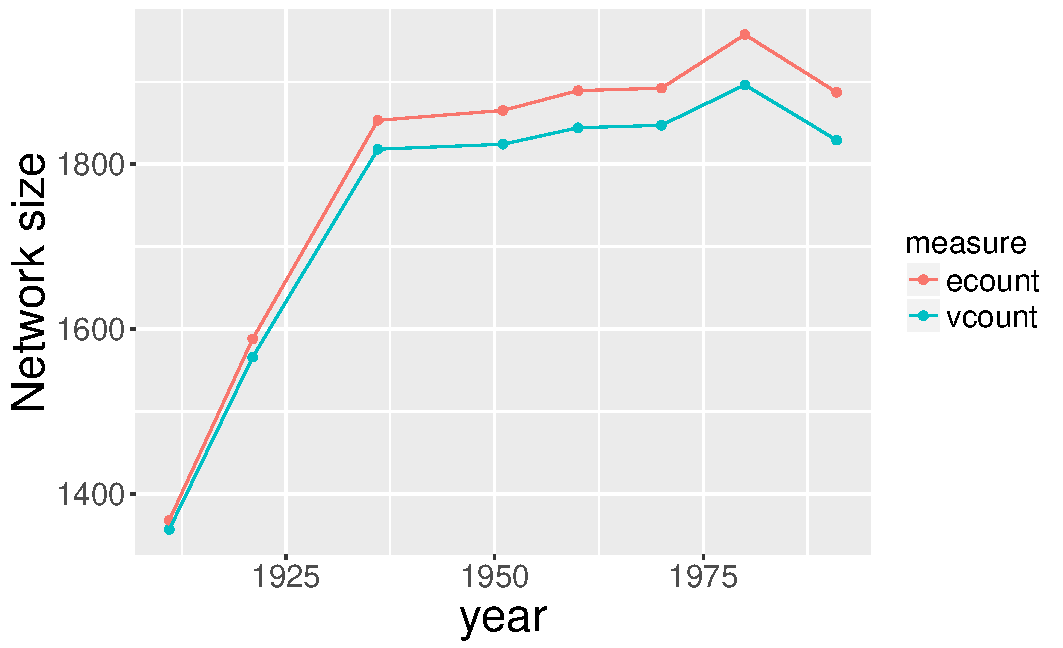
\includegraphics[width=0.4\textwidth]{figures/nw_nwSize}
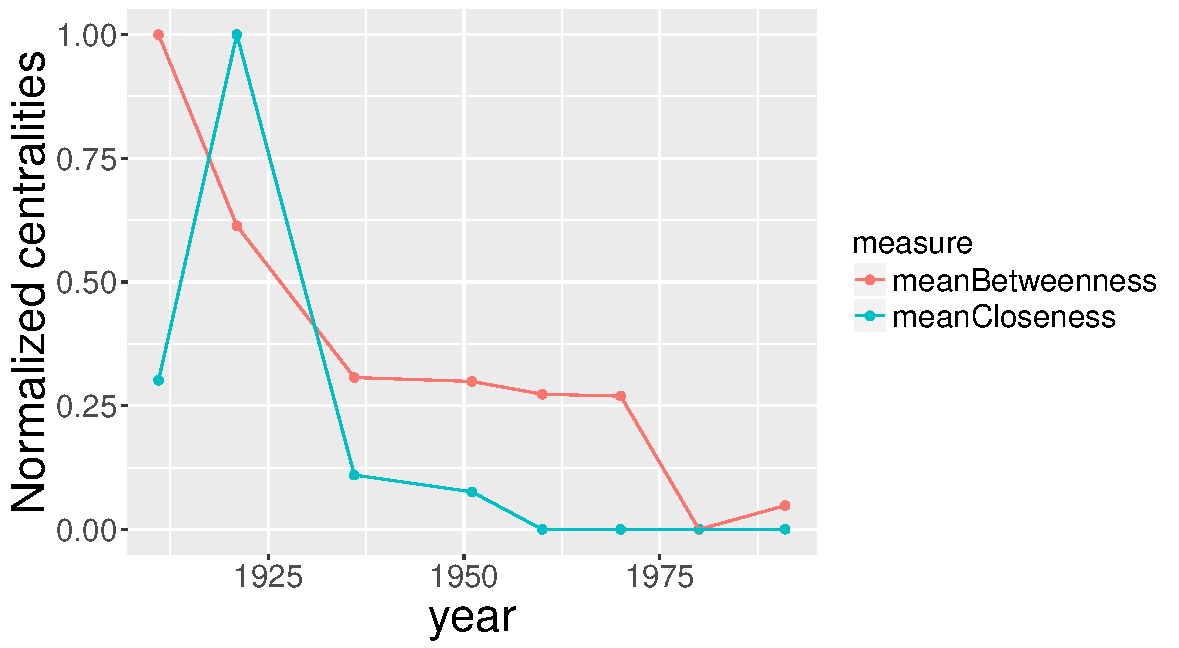
\includegraphics[width=0.45\textwidth]{figures/nw_meanCentralities}\\
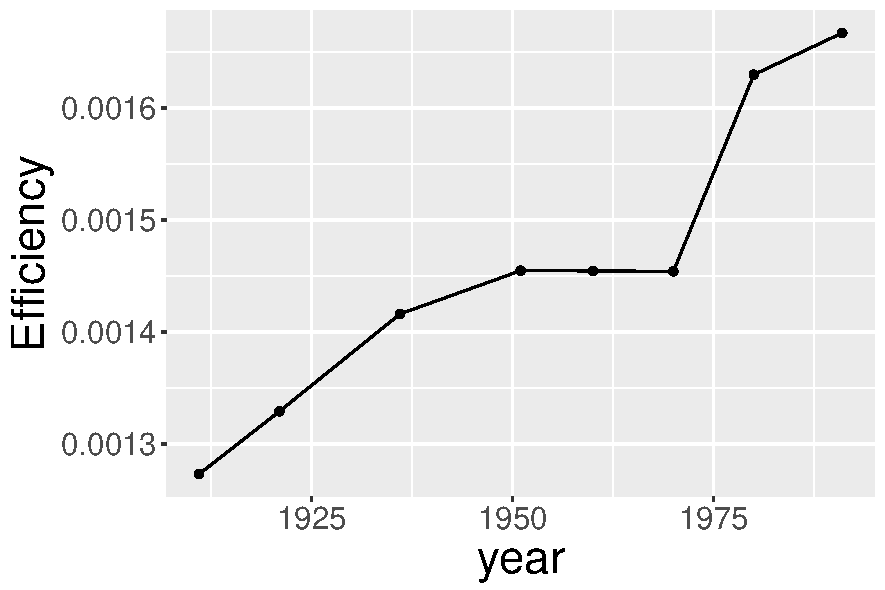
\includegraphics[width=0.4\textwidth]{figures/nw_efficiency}
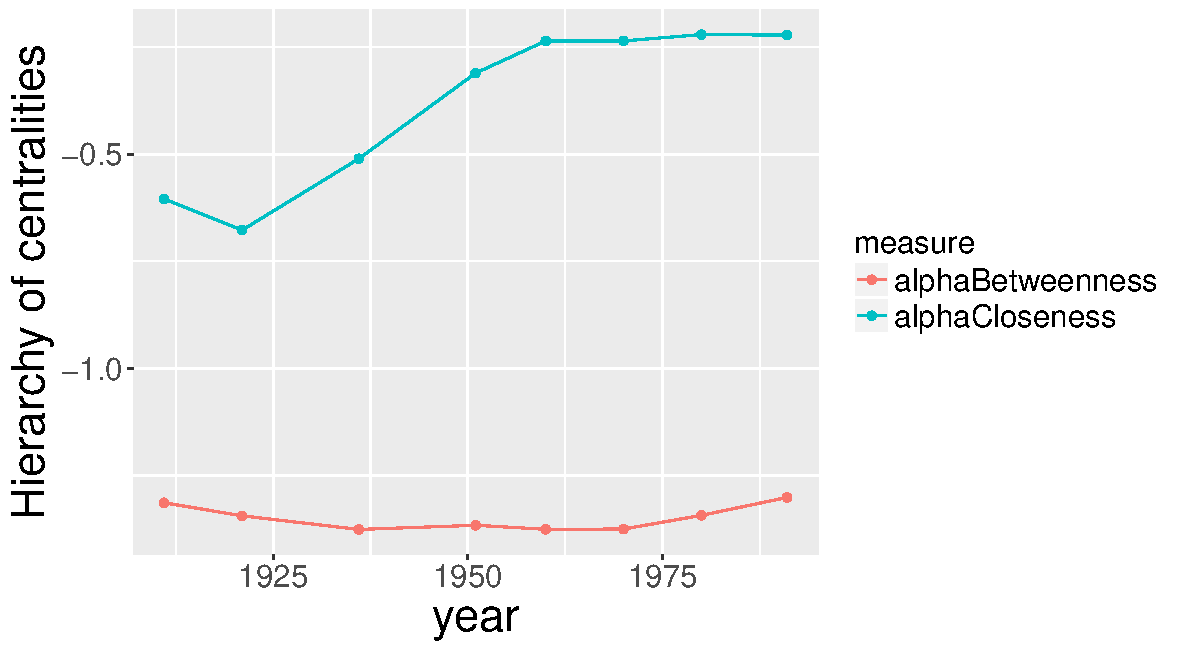
\includegraphics[width=0.45\textwidth]{figures/nw_hierarchies}


}



\sframe{Accessibility Patterns}{

\textit{A distorted co-evolution between the system of cities and the railway network}

\bigskip

\centering

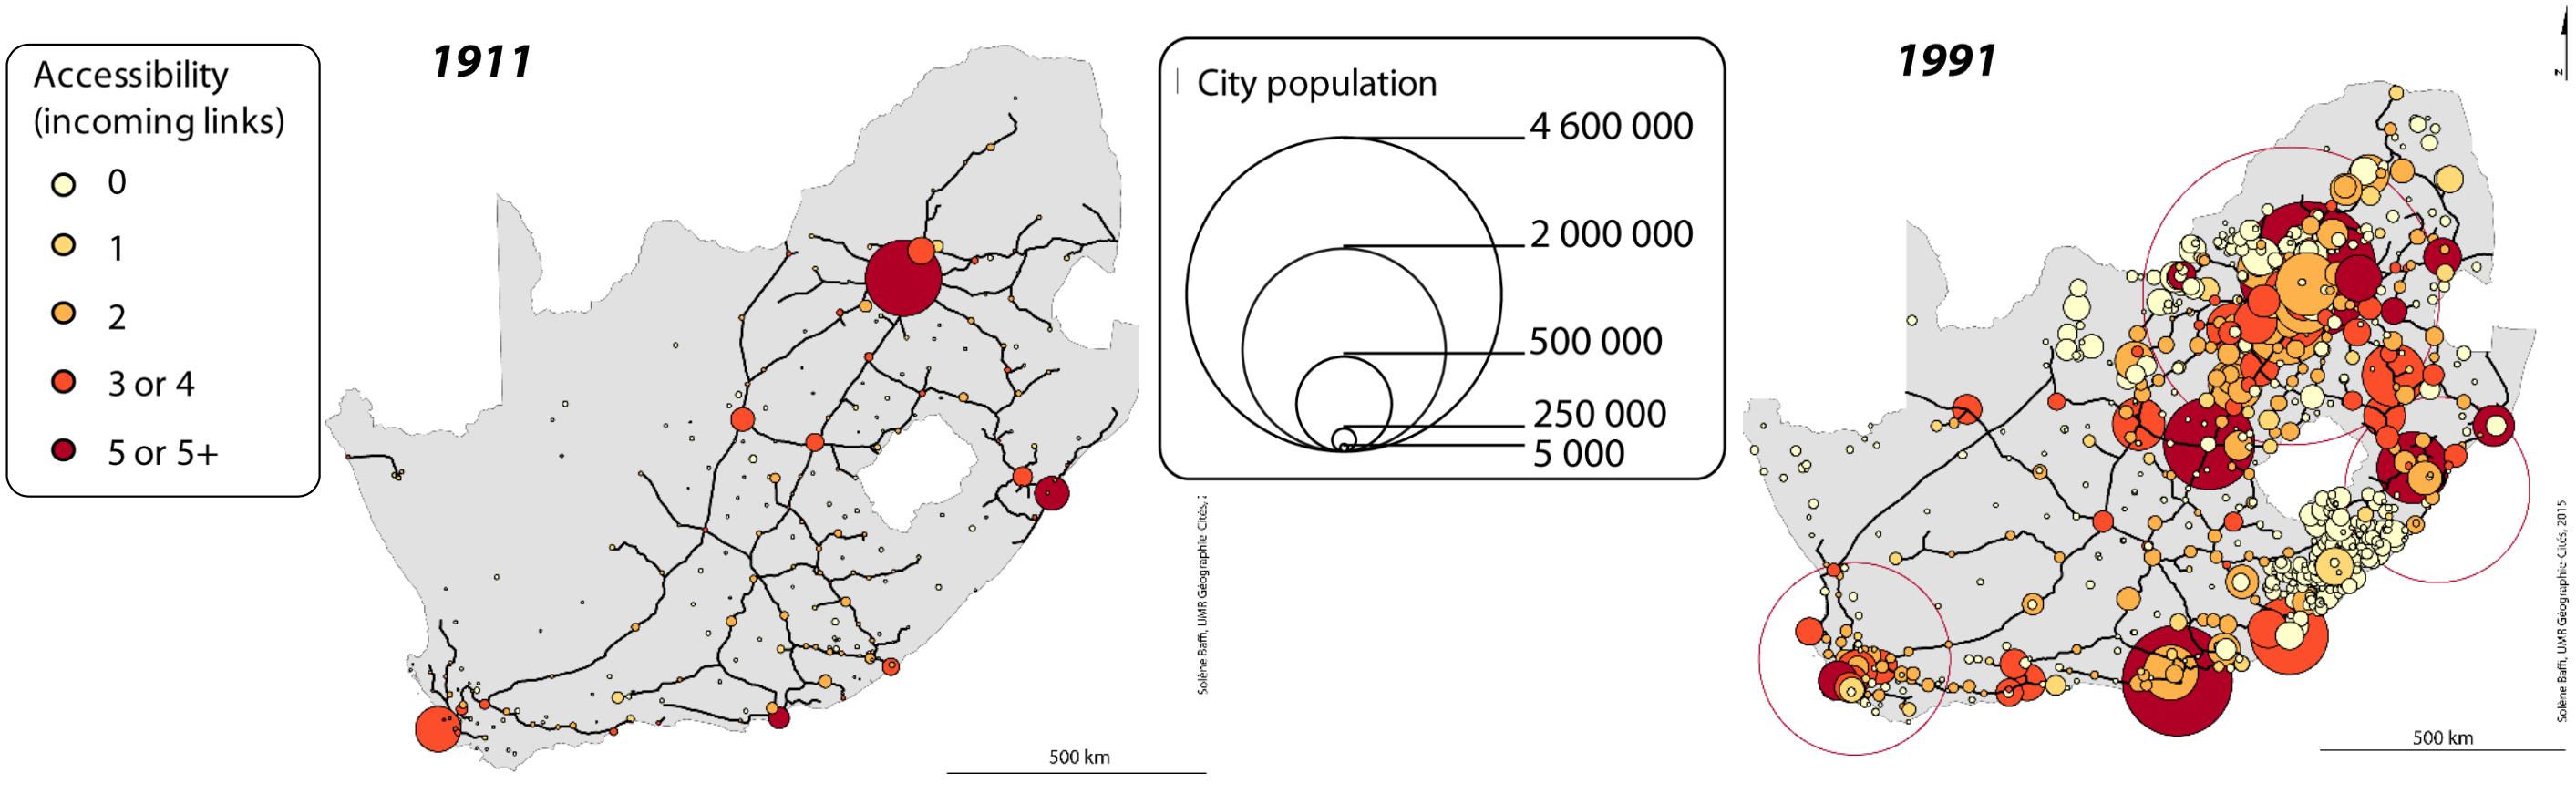
\includegraphics[width=\textwidth]{figures/accessibility-pop.png}


}


\sframe{Spatio-temporal causalities}{

}


\sframe{Stationarity scales}{

\textit{Optimal estimation time window and spatial range for accessibility}


\bigskip

\centering

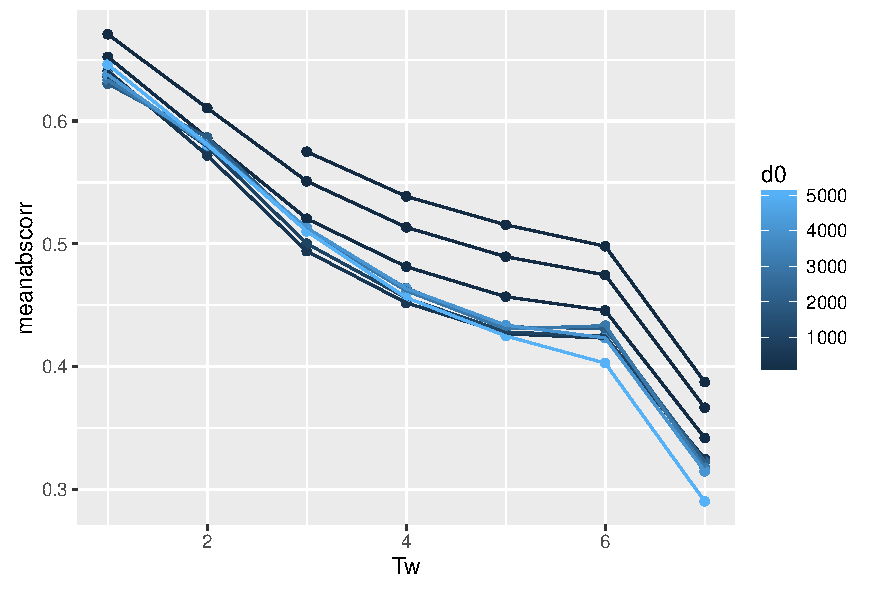
\includegraphics[width=0.5\textwidth]{figures/meanabscorrs}
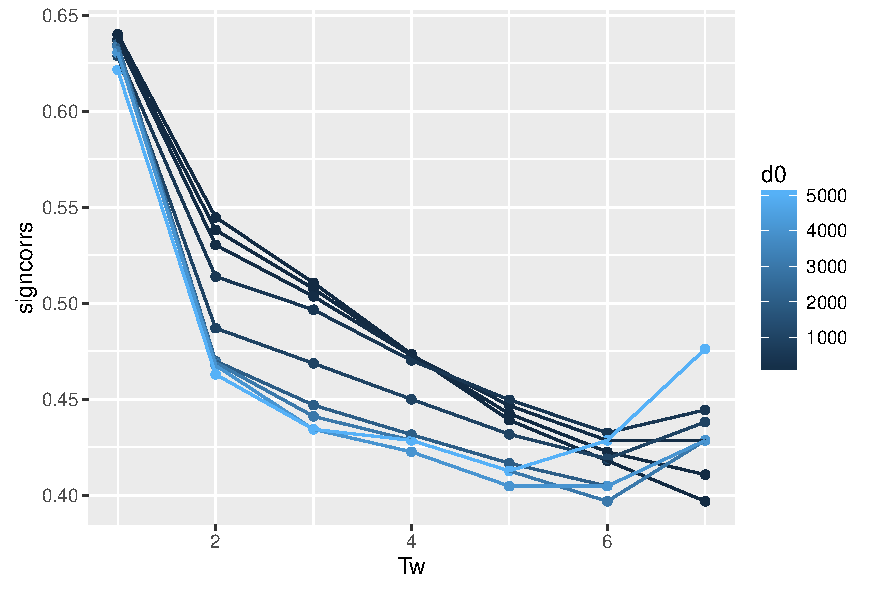
\includegraphics[width=0.5\textwidth]{figures/significantcorrs}

}


\sframe{Causality Patterns}{

\textit{Clear inversion of the sense of Granger causality suggests a structural segregation effect of the apartheid laws}

\bigskip

\centering

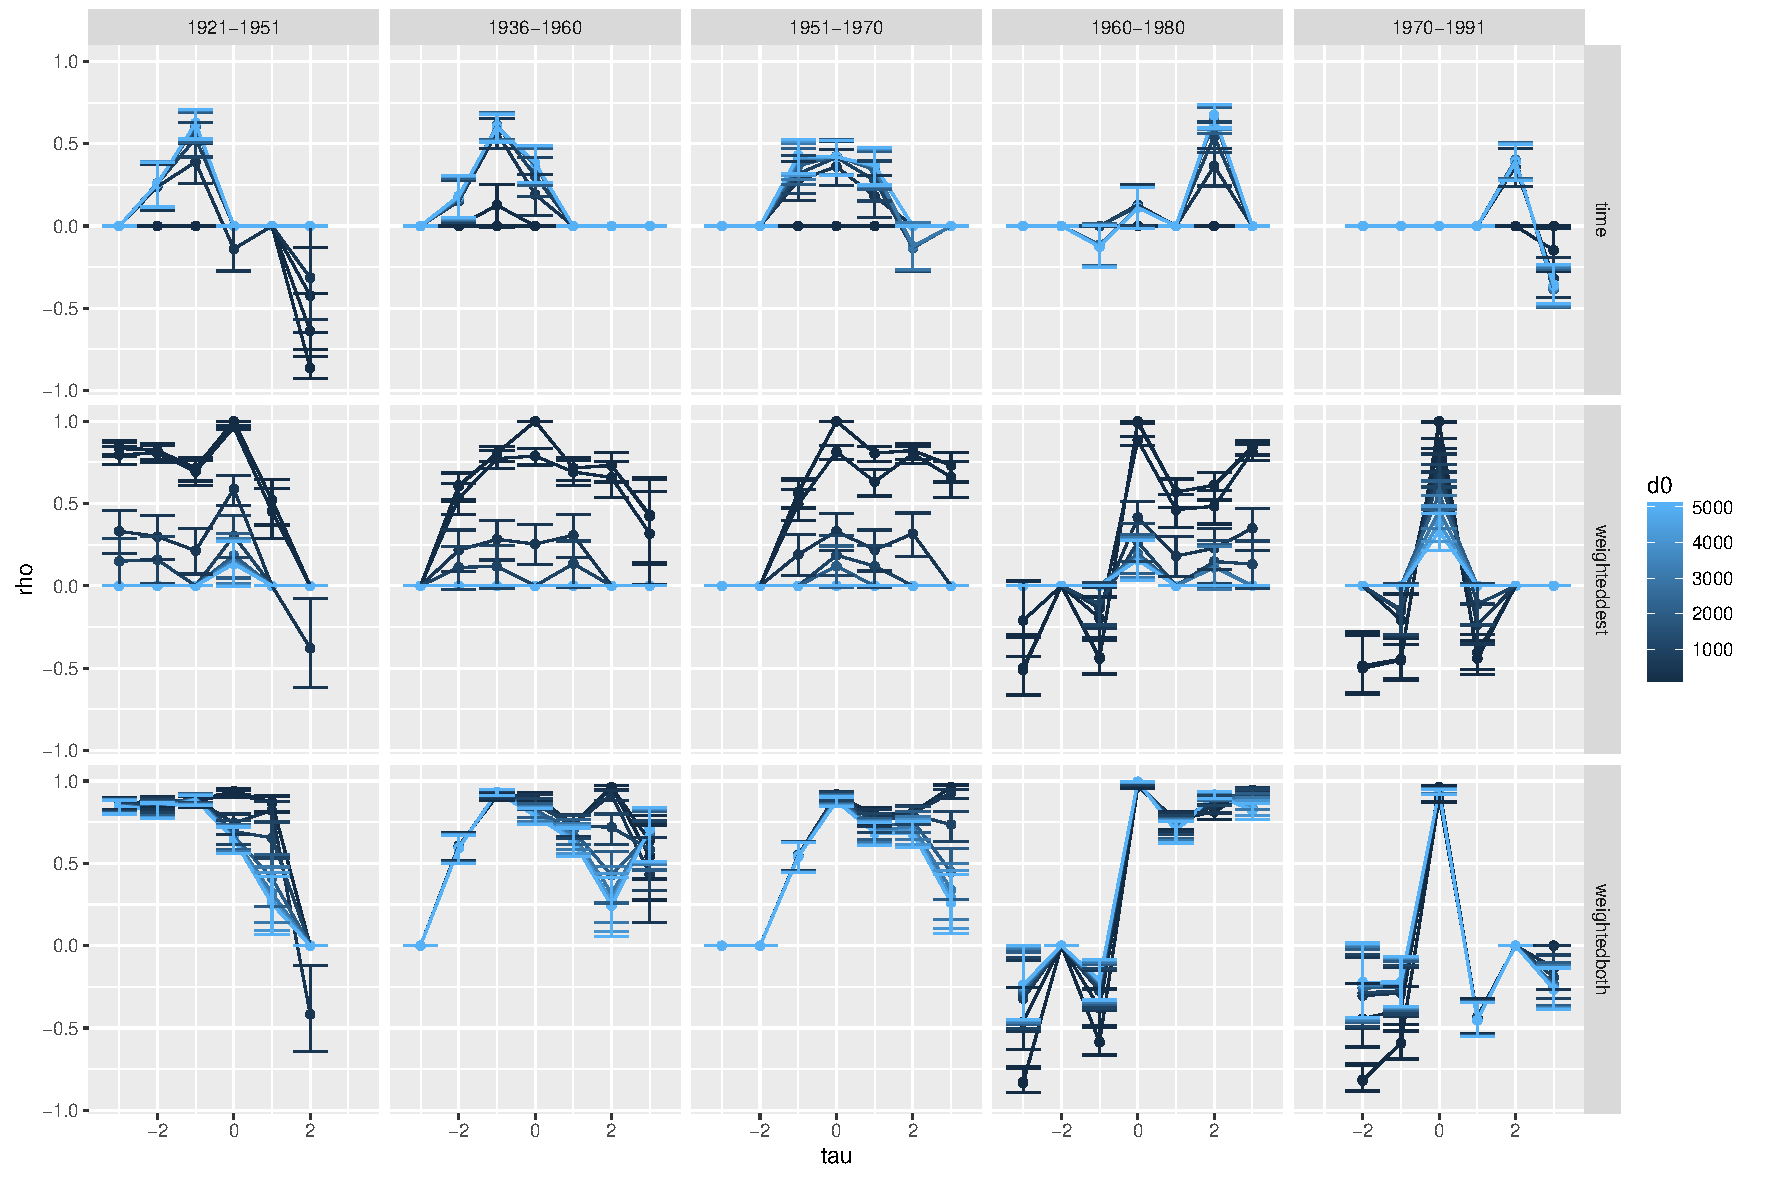
\includegraphics[width=0.82\textwidth]{figures/laggedCorrs_Tw3}

}


%%%%%%%%%%%%%%%%%
\section{Discussion}
%%%%%%%%%%%%%%%%%





\sframe{Discussion}{

\justify

\textbf{Implications}

$\rightarrow$ 

\bigskip

\textbf{Developments}

$\rightarrow$ 


}




\sframe{Conclusion}{

\justify

$\rightarrow$ 

\bigskip
\bigskip
\bigskip


\footnotesize{ - Code et data available at\\ \texttt{https://github.com/JusteRaimbault/CityNetwork/tree/master/Models/}
\\\texttt{SpatioTempCausality/SudAfrica}
}

}






\sframe{Reserve slides}{

\centering

\Large

\textbf{Reserve Slides}

}


\sframe{Defining co-evolution}{

}

\sframe{Database}{

}


\sframe{Accessibility}{

 $P_i$ populations, $d_{ij}$ network distance matrix, accessibility is given for $i$ by
  \[Z_i = w_i \sum_j w_j \exp \left(- d_{ij} / d_0 \right)\]
  with $d_0$ decay parameters and weights $w_i$ are $1/N$ or $P_i / \sum_j P_j$ depending on modality.
  
}


%%%%%%%%%%%%%%%%%%%%%
\begin{frame}[allowframebreaks]
\frametitle{References}
\bibliographystyle{apalike}
\bibliography{/Users/juste/ComplexSystems/CityNetwork/Biblio/Bibtex/CityNetwork,biblio}
\end{frame}
%%%%%%%%%%%%%%%%%%%%%%%%%%%%









\end{document}







